\section{Analysis}
We will start with characterizing some events by their visualized signature. Unfortunately, this is not sufficient to classify all events
properly, so in the next part we will conduct a more sophisticated analysis looking at the distribution of various variables 
measured by the detector. 

\subsection{Signatures of detected particles: Descriptive treatment}
On the next pages, figures~\ref{fig:ee},~\ref{fig:mm},~\ref{fig:tt} and~\ref{fig:qq} each show
a typical event corresponding to one particle. Although we will not use these figures any
further, they give an impression of what typical events look like.
The red curves indicate the data of the tracking detector, visualizing the trajectories
in the inner area. Pink squares indicate where the electron calorimeter measured energies
(denoted as $E_{\mathrm{ecal}}$)
with the blue squares showing their momentum. Green squares indicate the energy deposited in the
hadron calorimeter (called $E_{\mathrm{hcal}}$).

\begin{figure}[htpb]
    \centering
    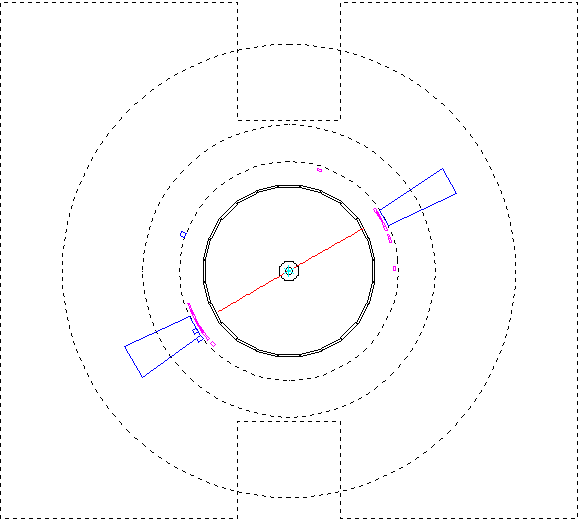
\includegraphics[width=0.8\linewidth]{figures/ee_02.png}
    \caption{Example for typical event of a decay into two electrons. The characteristic feature of the decay into electrons is
    the very little number of trajectories and most of the energy submitted to first calorimeter (in the inner circle).}
\label{fig:ee}
\end{figure}

\begin{figure}[htpb]
    \centering
    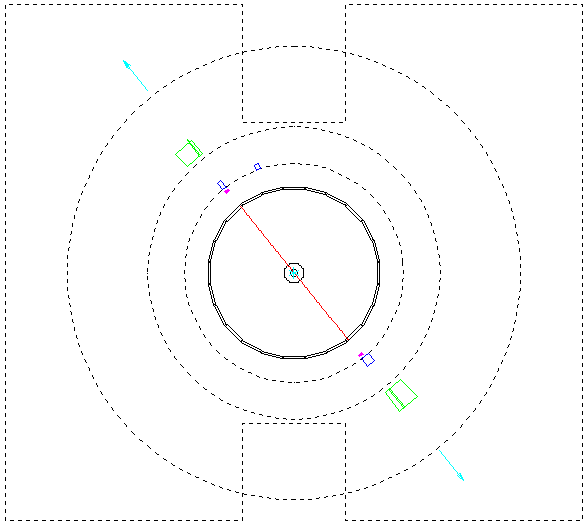
\includegraphics[width=0.8\linewidth]{figures/mm_02.png}
    \caption{Example for typical muon-muon decay. Due to the small interaction probability, 
        only little amounts of energy are absorbed by the first calorimeter. The muon detector lies outside of this pictures (which
    is indicated by the turquoise arrows). }
\label{fig:mm}
\end{figure}

\begin{figure}[htpb]
    \centering
    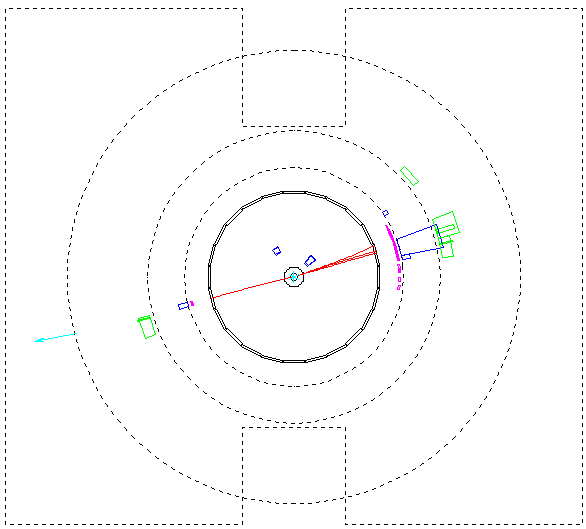
\includegraphics[width=0.8\linewidth]{figures/tt_02.png}
    \caption{Example for typical event of a decay into two tauons. As the particles are not
        stopped in the first calorimeter, the probability of being electrons decreases
        significantly (although this statement oversimplifies the reality, as we will see later). Furthermore,
        there is one particle escaping to the muon detector, but not two in opposite
        directions, as we would expect for muons. There are also no hadron showers
        as it would be characteristic for the quark branch. }
\label{fig:tt}
\end{figure}

\begin{figure}[htpb]
    \centering
    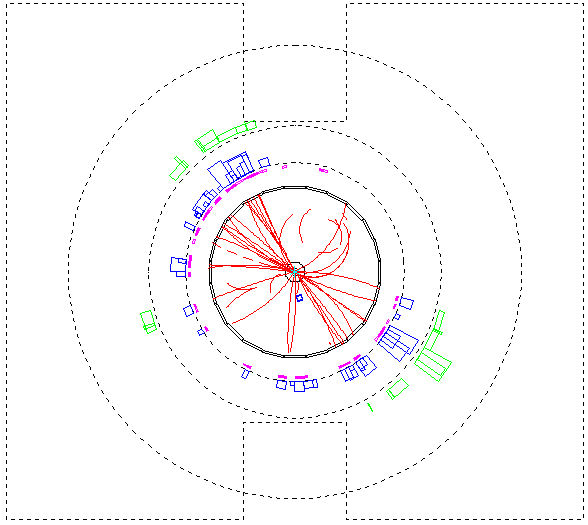
\includegraphics[width=0.8\linewidth]{figures/qq_02.png}
    \caption{Example for typical hadronic decay. As indicated in figure~\ref{fig:tt}, hadronic showers are 
   a signature for quarks, originating from the \textbf{strong confinement}. 
   As bound states of quarks can only be found at low enough
   momentum, we observe the creation of a large number of hadrons, being
   measured in both calorimeters. More than half of
   the energy carried by incident hadrons is passed to additional secondaries. }
\label{fig:qq}
\end{figure}

\clearpage
\subsection{Techniques used for the evaluation}
All calculations in this section are done with scripts written in 
the \textit{python} programming language~\cite{python}, relaying in several 
packages:
\begin{itemize}
    \item
        \textit{matplotlib}~\cite{Hunter2007} for plotting,
    \item
        \textit{scipy}~\cite{scipy} for fitting, and 
    \item
        \textit{uncertainties}~\cite{uc} for error propagation.
\end{itemize}
The latter applies Gaussian error propagation for correlated and uncorrelated variables. 
We will thus not explicitly write down the formulas for the error propagation 
for each quantity calculated but instead state the numerical result, only. 
We will, however make a quick remark on the use of covariance matrices in 
error propagation: Contrary to measured data, which in our case is usually 
expected to be uncorrelated, all fitted data yields variables that in general correlate. 
The propagation is then done as follows:
Let's assume we have random
variables $x_0,...,x_N$ which are correlated through the $N\times N$ Matrix $cov(x_i,x_j)$.
For a scalar function $f(x_0,...,x_N) \rightarrow \mathbb{R}$, the variance is estimated (linearly) by:
\begin{equation}
Var[f] = \sigma^2 = \sum_{i,j} \frac{\partial f}{\partial x_i} \frac{\partial f}{\partial x_j} cov(x_i,x_j) \,.
\end{equation} 
If instead, $\mathbf{f}$ is a vector field in $m$ dimensions, namely 
$\mathbf{f}(x_0,...,x_N) \rightarrow \mathbb{R}^m$, then the components of $\mathbf{f}$ 
are further correlated. We can write down the relation between the covariance matrices $V$ and $U$ of 
$\mathbf{x}$ and $\mathbf{f}$, respectively, in matrix relations:
\begin{equation}
    U = A V A^T
\end{equation}
where $A$ is the matrix defined by 
\begin{equation}
    A_{ij} = \left[ \frac{\partial f_i}{\partial x_j}\right]_{\mathbf{x} = \mu}
\end{equation}
with expectation value $E[\mathbf{x}] = \mu$.~\cite{cowan1998statistical}
In order to facilitate notation, the covariance matrices will in general be notated without 
specifying the units. If not specified explicitly, the units will correspond to those of the
variables: If $x_i, x_j$ have the units $[x_i], [x_j]$, respectively, 
then the entry of the covariance matrix has the unit $[x_i] \cdot [x_j]$. 

\clearpage

\subsection{Machine learning for classification}
As it is shown in section~\ref{sub:montecarlo},
the distributions of the different particles intersect in terms of different
variables. This makes the task of differentiating between particle types in the 
data a highly non-trivial one. We therefore searched for various techniques in order
to improve the classification of the particle species, seeking success using, inter alia, machine learning. 
As mentioned before, the analysis is done within the python
ecosystem. In particular, for the machine learning algorithms we use the library 
\textbf{scikit-learn}~\cite{scikit-learn}. 
The technique which we will present
here is used for our evaluation and turned out to be the best solution for our problem.
It is called \textbf{k-nearest neighbors algorithm} and
widely used in pattern recognition, because it is a non-parametric method\footnote{
We rely on non-parametric statistics because we do not know the probability distributions 
in the variables for the different particle species.
The number of parameters used in non-parametric techniques depends on the applied training set. 
This is unlike in parametric methods, where this number is fixed. This is often successful when the boundary is rather irregular.} 
which can be implemented easily. For details on the implementation, please refer to the appendix~\ref{sub:cut.py}.
\begin{SCfigure}
    \centering
    \caption{The \textbf{k-nearest neighbors algorithm} works as follows: 
        The algorithm stores all instances of the training data and their respective
    classification \textit{(colored bubbles)}. When classifying a new instance \textit{(bubble with question mark)}, the 
    predictor counts how many nearest neighbors of the unknown instance are of a specific type. 
    Depending on the parameter \textbf{k}, the point is assigned the class of the majority. 
    In the beginning, when only the learning set is available,
    the parameter \textbf{k} is chosen such that the error of second order is minimized. In general, a larger \textbf{k} will
    limit the effects of stochastic noise but make the classification boundaries fuzzier.}
    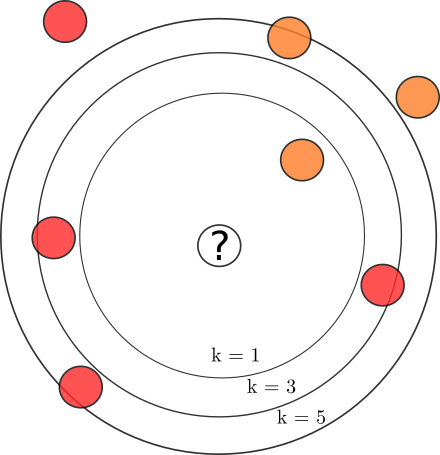
\includegraphics[width=0.5\linewidth]{figures/knn_schema}
\label{fig:knn_schema}
\end{SCfigure}

\begin{figure}[htpb]
    \centering
    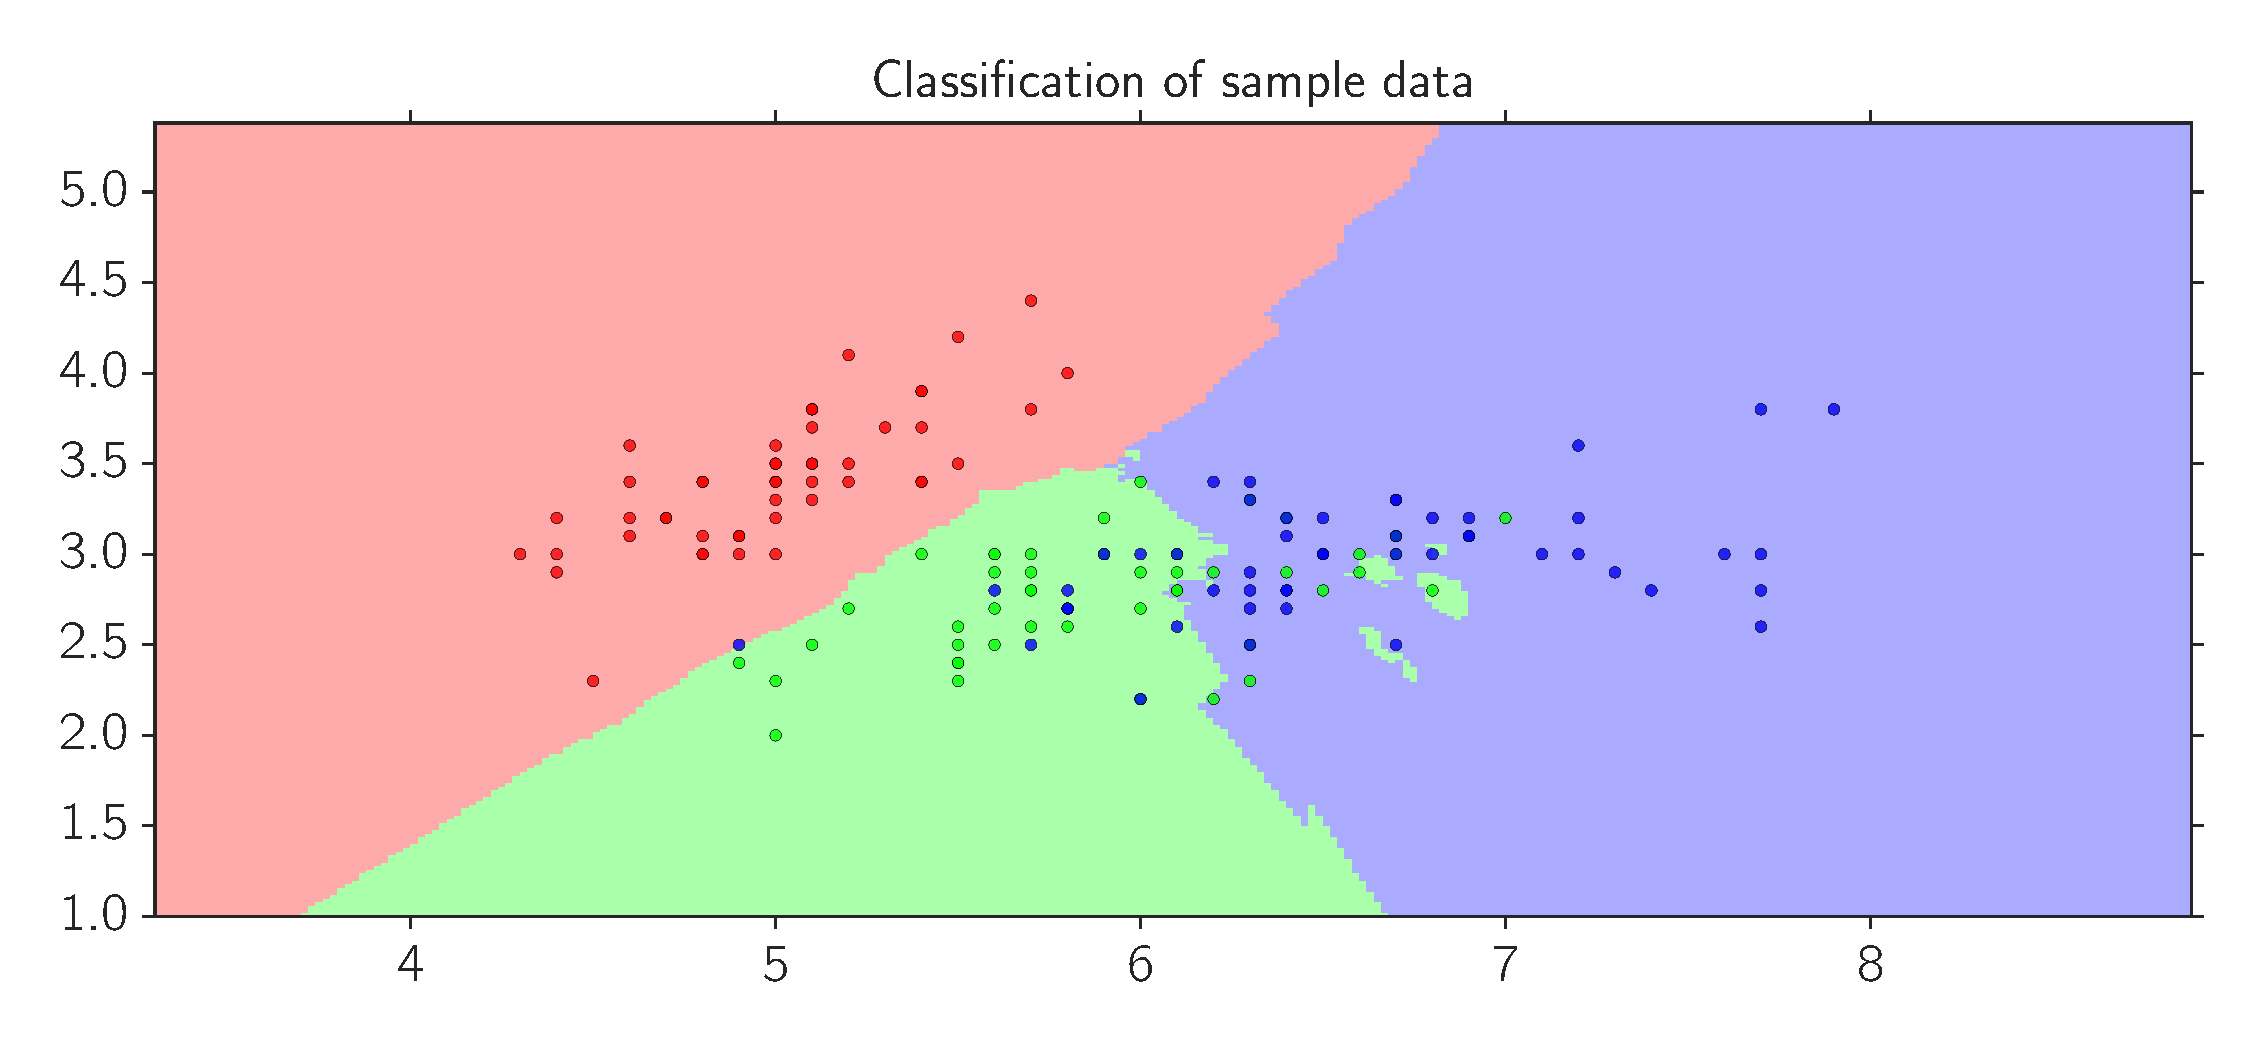
\includegraphics[width=1\linewidth]{figures/kneigbors}
    \caption{Example taken from documentary of \textbf{scikit-learn}\cite{scikit-learn}, the library we are using. One x can
    see the learning data \textit{colored dots} and the prediction for homogeneously distributed test data
    (\textit{colored surface}) plotted. The data is the \textit{Iris flower data set} \cite{frank1968numerical}, commonly used 
    in order to benchmark a supervised learning algorithm. For a detailed examples of \textbf{scikit learn}
    refer to \cite{masteringscikit}.}
\label{fig:kneigbors}
\end{figure}

\clearpage
\subsection{Monte Carlo data}

\label{sub:montecarlo}
In order to get an intuition about the distributions governing the different particle species with respect to the measured
variables, we use Monte Carlo generated data. These do not come in the correct branching ratios. For the following histograms 
as well as the analysis of our algorithm, we rescale the corresponding numbers of events to match branching ration given 
in the literature, ~\cite{pdg}. Furthermore, our preparation with the simulated data is limited by the fact that these are 
only available for one energy each, all close to 91.2 GeV.  
What is clearly visible in figure \ref{fig:cos_figs}, \ref{fig:monte1} and \ref{fig:monte2} is that the
different particle species are not separable in terms of the single variables completely. This is why we use a 
\textit{non parametric} method in order to classify the particle species, since the hypersurfaces separating the distributions
might be of a non trivial geometric shape, possibly including highly non linear parametrization. 
Furthermore, the probability distribution are not linear in the respective variables and can be visualized best on a logarithmic 
scale.
\begin{figure}[htpb]
    \centering
    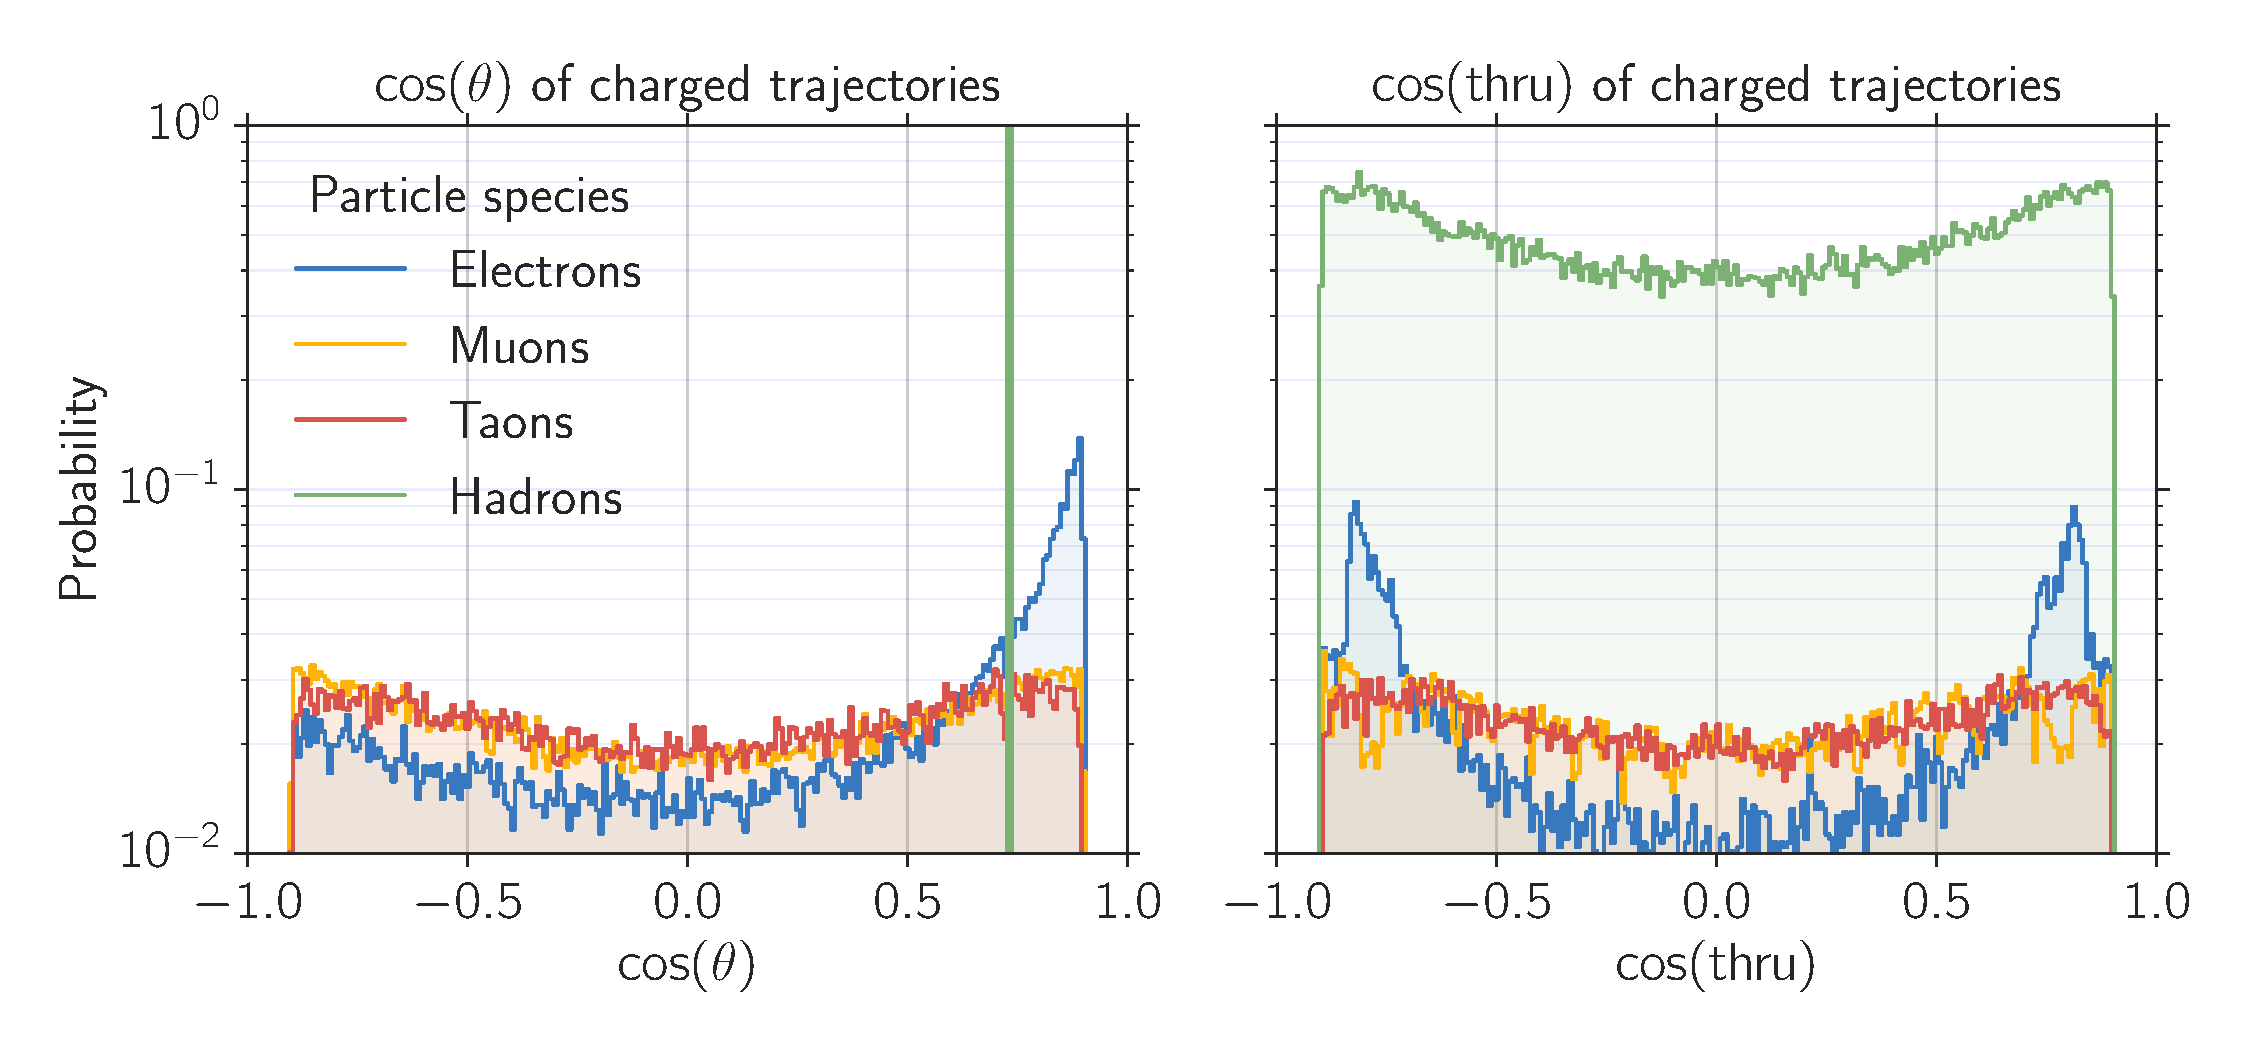
\includegraphics[width=1.0\linewidth]{figures/cos_figs}
    \caption{Distribution of the Monte Carlo data (with correct branching ratios) 
    with respect to the $\cos(\theta)$ and $\cos(\mathrm{thru})$. Note that $\cos(\theta)$ is not defined properly
    for hadrons. Later, when classifying
    real data, this is not as clear as it is here, forcing us to exclude not well defined variables from the classification process.
    Another observation is the absence of the t-channel in particle species other than electrons. This simplifies 
    the classification process enormously, because in this case the chronological 
    order of removing the t-channel is not as crucial to the particle numbers.}
    \label{fig:cos_figs}
\end{figure}

\begin{figure}[htpb]
    \centering
    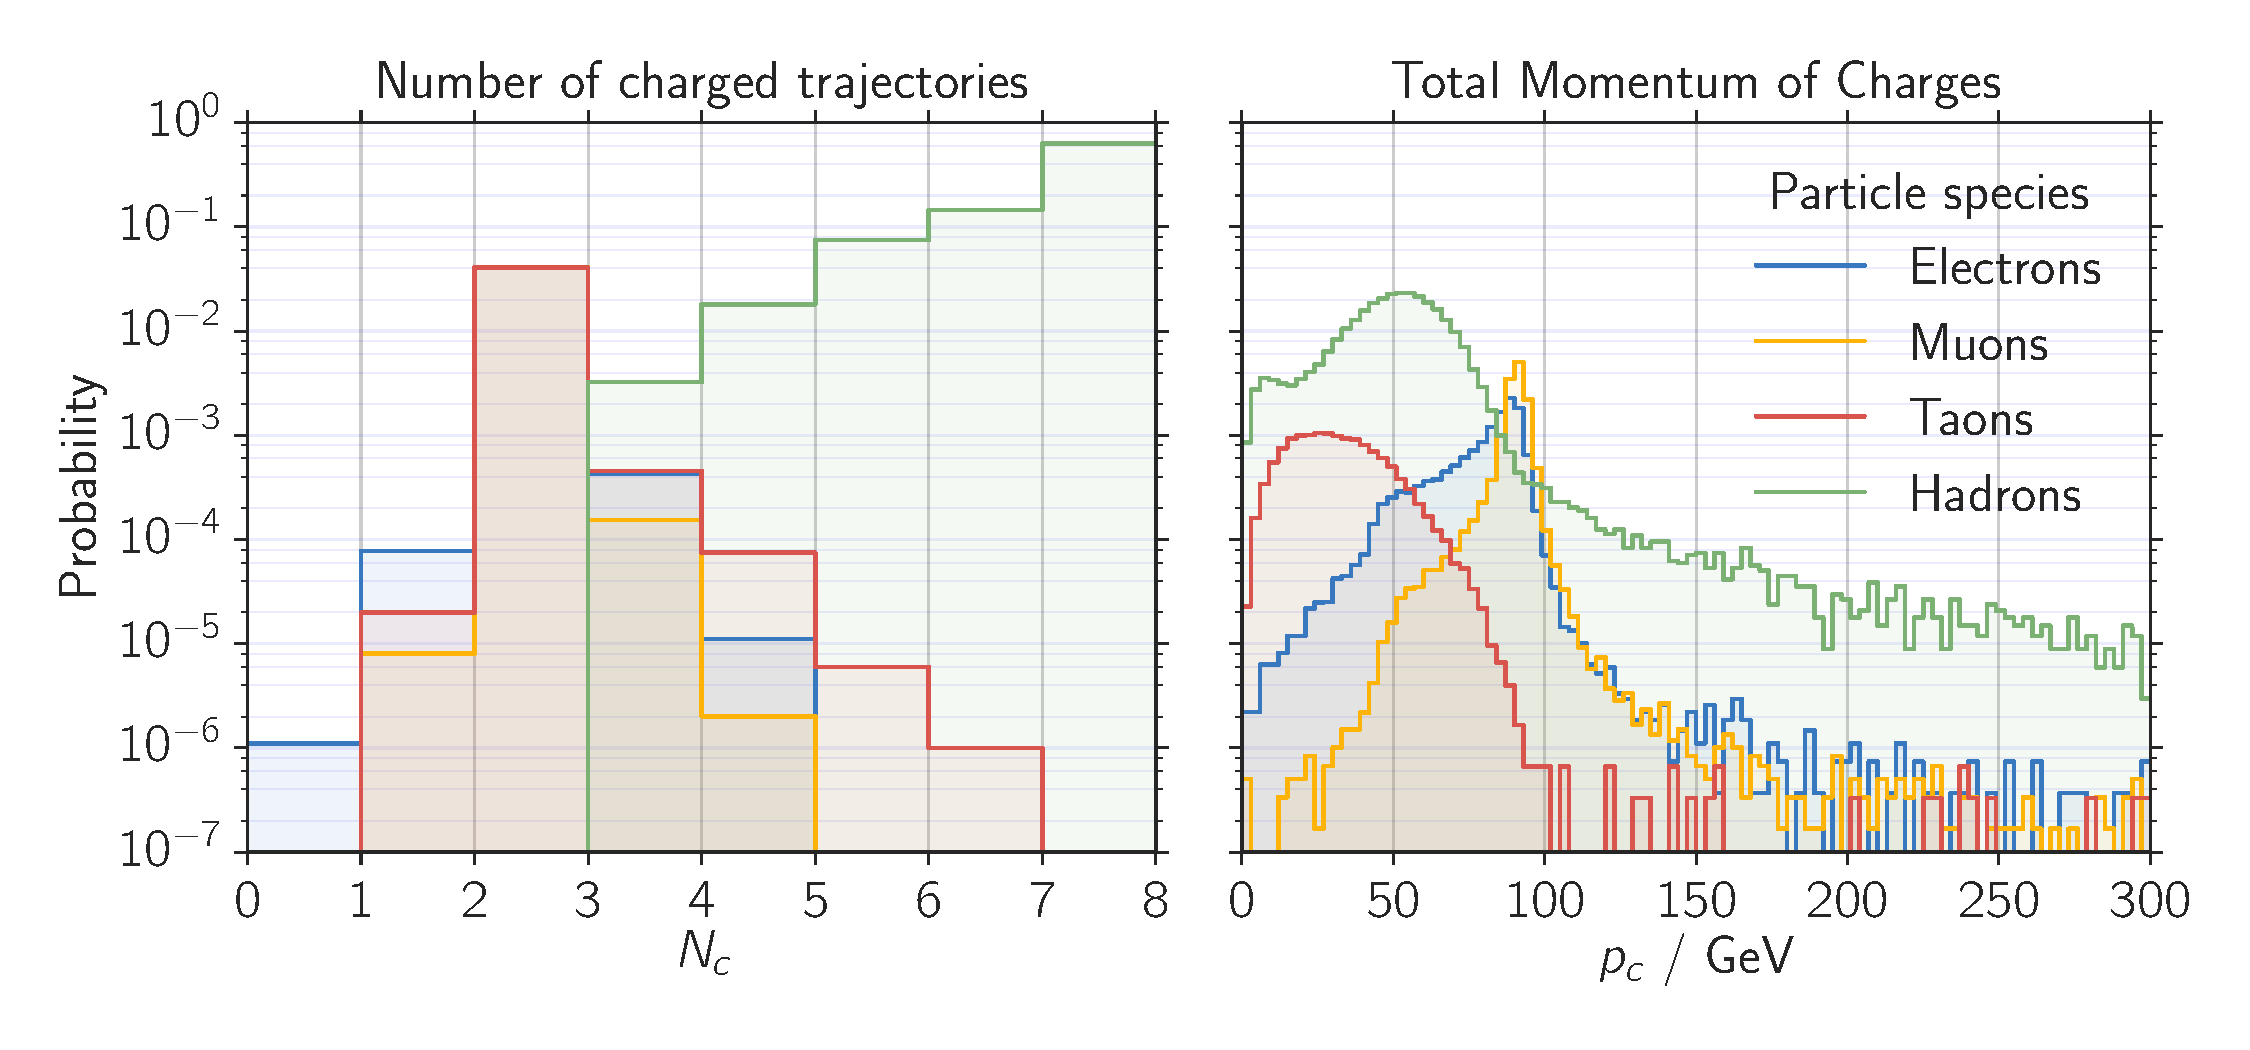
\includegraphics[width=1.0\linewidth]{figures/N_p_c}
    \caption{Distributions of Monte Carlo data (with correct branching ratios)
        over (a) the number of measured trajectories $N_c$ and (b) the total charged
        momentum $p_c$.Note the logarithmic scale. 
        For $N_c$, overlap exists from one to seven trajectories. The hadron's distribution 
        continues with non-zero probability up to $N_c = 55$ (not shown). }
    \label{fig:monte1}
    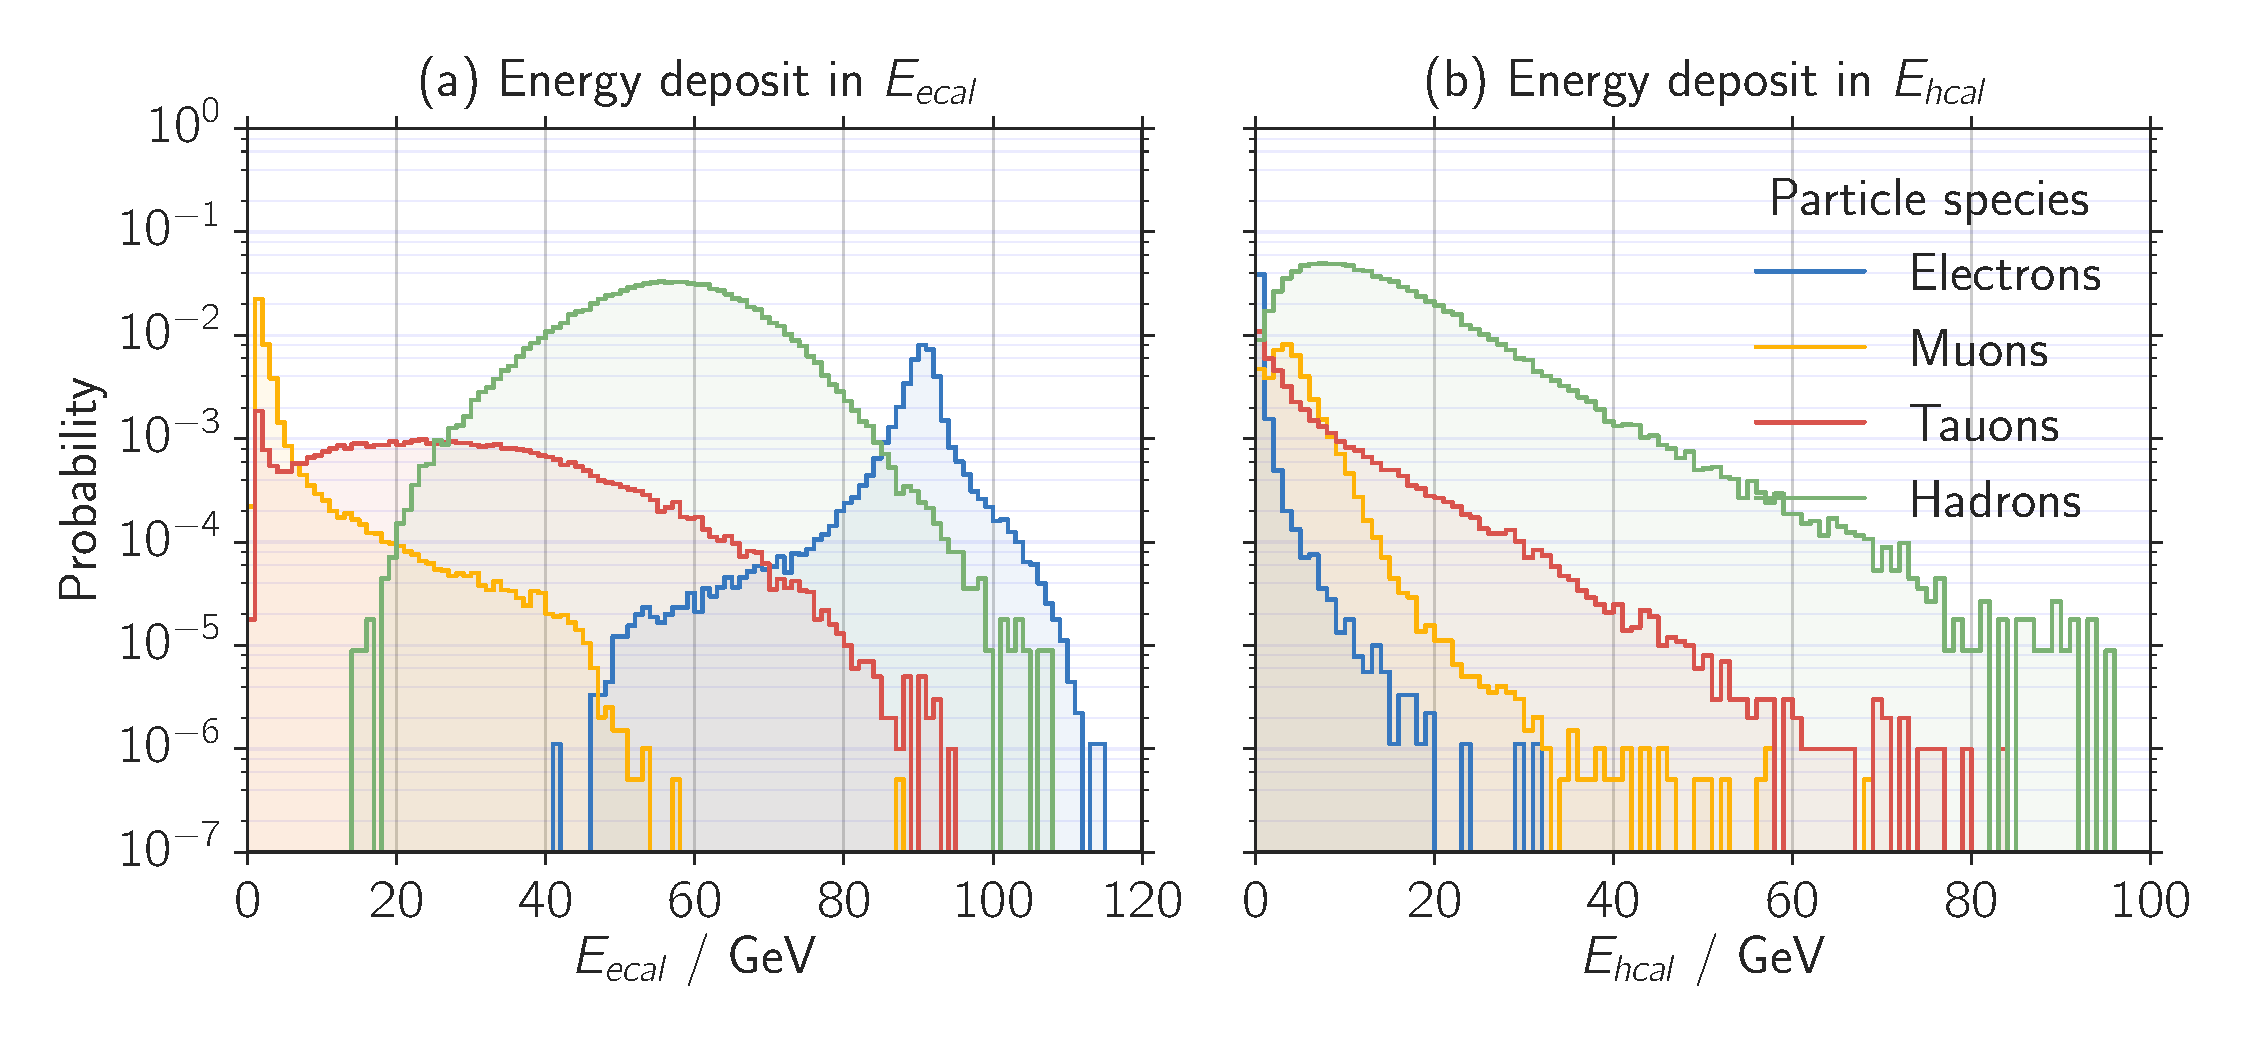
\includegraphics[width=1.0\linewidth]{figures/E_cal}
    \caption{As in the figure above, but in in the variables $E_{ecal}$ and $E_{hcal}$ 
        (energy deposit in electron and hadron calorimeter, respectively). Notice the separation between electrons
    and muons in (a), but the overlap with tauons in all regimes.}
\label{fig:monte2}
\end{figure}

\clearpage
\subsubsection{Fitting t/s-channel}
\label{ssub:FittingTsChannel}
In section \ref{sub:bhabha} we explain that the t-channel of the electronic decay does not correspond
to the cross section of the process we are interested in. Hence we need to remove it.  The equation governing 
the $\cos(\theta)$ distribution of electrons looks as following
\begin{equation*}
\sigma_{ee} = A(1 + \cos^2\theta) + B(1 - \cos\theta)^{-2}.
\end{equation*}
Fitting this function to the real data, we can remove the s-channel easily, as seen in figure \ref{fig:tschannel}.
\begin{figure}[htpb]
    \centering
    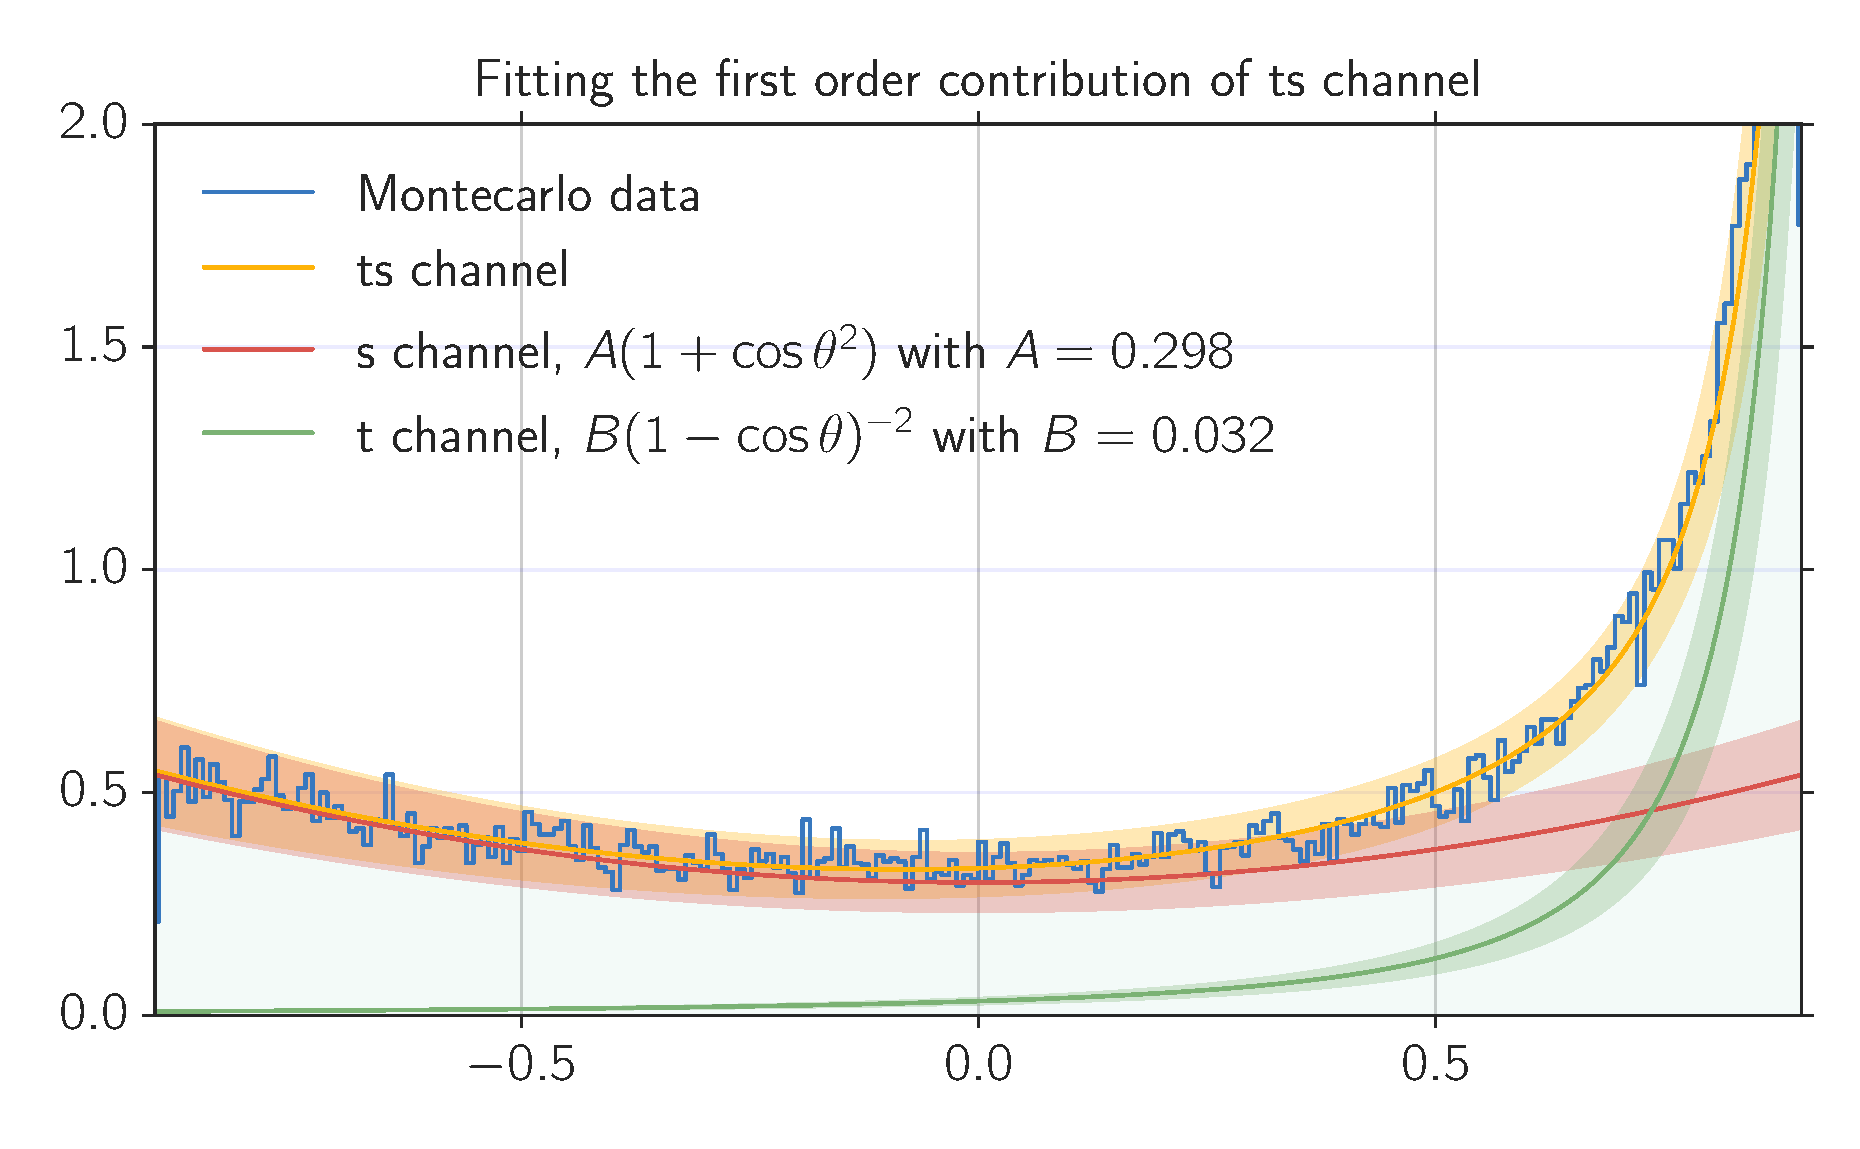
\includegraphics[width=1.0\linewidth]{figures/tschannel}
    \caption{Removing the t-channel from the electron data. 
        We apply a fit of the data in order to be able to subtract the t-channel. What remain are
    the electrons in the s-channel. This figure is an illustration of the method using Monte Carlo data. It is
    applied to real data later on.}
    \label{fig:tschannel}
\end{figure}
\clearpage

\subsubsection{Efficiency matrix}
\label{ssub:Efficiencymatrix}

The first step in classifying the real data is to assign single events to a specific decay branch in order to
compare the different distributions. The problem is that wrong assignments will lead to wrong contributions 
in the final cross-section. Therefore a good strategy is to test the classification algorithm with Monte Carlo data and 
quantify its efficiency. We correct the systematic error contribution of the algorithm afterwards. First we 
divide the Monte Carlo data in a training sample (75\% of the data) and a test sample (25\% of the data) to avoid
inconsistent testing.  At this point we tried different algorithms. The efficiency of the algorithms based on the training
data is shown in table \ref{tab:eff1} (where we used physical intuition to separate the particle species) and in table
\ref{tab:eff2} (where we used the machine learning technique \textit{k-nearest neighbors algorithm}). As these tables indicate,
the machine learning technique was far more successful with respect to efficiency, so we used this one for the further 
calculations. \\
The efficiency matrices show, which (true) particles were classified falsely into which species. The correction
of the real data is done with the inverse of this matrix:
\begin{equation}
    \label{eq:eff_inverse}
    N_{\mathrm{True}} = N_{ \mathrm{observed}} \cdot M_{\mathrm{eff}}^{-1}
\end{equation}


\begin{table}[htpb]
    \centering
    \caption[caption]{Efficiency matrix $M_{\mathrm{eff}}$ with \textbf{physical intuition}\footnotemark.}
    \label{tab:eff1}
\begin{tabular}{l| l| l| l |l}
\rowcolor{LightCyan} & Electrons & muons & Tauons & Hadrons \\ 
    \cellcolor{LightCyan} Electrons & $\mathbf{0.9571 \pm 0.1722}$ & $0.0000 \pm 0.0000$ & $0.0087 \pm 0.0013$ & $0.0050 \pm 0.0005$ \\ 
    \cellcolor{LightCyan} Muons & $0.0000 \pm 0.0000$ & $\mathbf{0.9285 \pm 0.0093}$ & $0.0530 \pm 0.0018$ & $0.0010 \pm 0.0002$ \\ 
    \cellcolor{LightCyan} Tauons & $0.1628 \pm 0.0217$ & $0.0637 \pm 0.0018$ & $\mathbf{0.9247 \pm 0.0101}$ & $0.0294 \pm 0.0012$ \\ 
    \cellcolor{LightCyan} Hadrons & $0.0000 \pm 0.0000$ & $0.0000 \pm 0.0000$ & $0.0018 \pm 0.0003$ & $\mathbf{0.9508 \pm 0.0092}$ \\
\end{tabular}
\end{table}
\footnotetext{We tried the following setup here:\\
\begin{tabular}{l| l| l | l }
    Electrons & $60<E_{\mathrm{cal}}<120 $ & $40 < P_{\mathrm{charged}} < 100 $ &$0 <N_{\mathrm{charged} }< 10$ \\ 
    Muons & $0 <E_{\mathrm{cal}}<40 $ &$60 < P_{\mathrm{charged}} < 120 $ & $0 <N_{\mathrm{charged} }< 10$\\ 
    Tauons & $0<E_{\mathrm{cal}}<100 $ &$ 0  < P_{\mathrm{charged}} < 100 $& $0 <N_{\mathrm{charged} }< 40$\\ 
    Hadrons & $20<E_{\mathrm{cal}}<100 $ & $0  < P_{\mathrm{charged}} < 100 $& $ 10 <N_{\mathrm{charged} }$
\end{tabular}\\
As we do not use this cut method in the further analysis, we will not comment on the choice of parameters here anymore, for 
a visualization of the distributions see figure \ref{fig:monte1} and \ref{fig:monte2}. 
% There is not much space for the table, but vspace is not working here, I have no idea how to fix this.
}
\begin{table}[htpb]
    \centering
    \caption{Efficiency matrix $M_{\mathrm{eff}}$ with \textbf{k-nearest neighbors algorithm}}
    \label{tab:eff2}
\begin{tabular}{l| l| l| l |l}
\rowcolor{LightCyan} & Electrons & Muons & Tauons & Hadrons \\ 
    \cellcolor{LightCyan} Electrons & $\mathbf{0.9967 \pm 0.1931}$ & $0.0001 \pm 0.0001$ & $0.0026 \pm 0.0013$ & $0.0004 \pm 0.0001$ \\ 
    \cellcolor{LightCyan} Muons & $0.0000 \pm 0.0000$ & $\mathbf{0.9850 \pm 0.0097}$ & $0.0136 \pm 0.0009$ & $0.0001 \pm 0.0001$ \\ 
    \cellcolor{LightCyan} Tauons & $0.0181 \pm 0.0030$ & $0.0147 \pm 0.0008$ & $\mathbf{0.9717 \pm 0.0104}$ & $0.0031 \pm 0.0004$ \\ 
    \cellcolor{LightCyan} Hadrons & $0.0024 \pm 0.0007$ & $0.0001 \pm 0.0001$ & $0.0056 \pm 0.0006$ & $\mathbf{0.9964 \pm 0.0096}$ \\
\end{tabular}
\end{table}
\clearpage
\subsection{OPAL data}
\label{sub:opal_data}
The data used in this experiment is a set of 141144 events of seven different runs of 
the LEP accelerator. The corresponding center of mass energies and number of events are listed in 
table~\ref{tab:event_data}. Each event is characterized by values of variables measured 
by the OPAL detector. The variables we use in our 
analysis are summed summed up in table~\ref{tab:vars}. To assign a particle species 
to each event, we used to machine learning algorithm previously trained and analyzed 
on the Monte Carlo data. The events identified as electrons then undergo the procedure 
of removing the t-channel share, as described in section \ref{ssub:FittingTsChannel}.
The fitting is done separately for different beam energies $E_\mathrm{lep}$, because 
the proportion of the t-channel strongly depends on this variable. 
For low energies, it constitutes as much as 90\% of the t/s-channel.
The results of this procedure are summarized in table BLABLABLA. 
Finally the obtained numbers of events in each category and for each beam energy 
are then rescaled by the inverse efficiency matrix, see equation~\eqref{eq:eff_inverse}.

\begin{table}[htpb]
    \centering
    \caption{OPAL data from seven different runs. For each run, there are $N_\mathrm{run}$ events with a mean center of mass 
        energy $\overline{\sqrt{s}}$, where $\sqrt{s} = 2 E_\mathrm{lep}$. The standard deviation of 
    $\sqrt{s}$ indicates the low differences of beam energy within one run. }
    \label{tab:event_data}
    \begin{tabular}{l l c c}
        \rowcolor{LightCyan}Run & $N_\mathrm{run}$ & $\overline{\sqrt{s}}$ / GeV & std\_dev($\overline{\sqrt{s}}$) / GeV \\
        \cellcolor{LightCyan}$1$& 4332 & 88.483 & 0.009   \\
        \cellcolor{LightCyan}$2$& 9747 & 89.476 & 0.020   \\
        \cellcolor{LightCyan}$3$& 11507 & 90.234 & 0.013   \\
        \cellcolor{LightCyan}$4$& 82009 & 91.167 & 0.059   \\
        \cellcolor{LightCyan}$5$& 16043 & 91.988 & 0.022   \\
        \cellcolor{LightCyan}$6$& 8065 & 92.971 & 0.008   \\
        \cellcolor{LightCyan}$7$& 9441 & 93.729 & 0.013   \\
    \end{tabular}
\end{table}

\begin{table}[htpb]
    \centering
    \caption{Table of variables used in analysis}
    \label{tab:vars}
    \begin{tabular}{l|l}
  \rowcolor{LightCyan} Name & Meaning \\ 
    $N_{\mathrm{charged} }$ & Number of charged trajectories \\
    $P_{\mathrm{charged} }$ & Total momentum of charged trajectories \\
    $E_{\mathrm{ecal}}$ & Energy stored in electronic calorimeter \\
    $E_{\mathrm{hcal}}$ & Energy stored in hadronic calorimeter \\
    $E_{\mathrm{lep}}$ & Total energy (center of mass energy) \\
    $\cos\theta$ & Scattering angle of single trajectories \\
    $\cos\mathrm{thru} $ & Spread of the jet (merely hadrons)\\
    \end{tabular}
\end{table}






We continue by calculating the cross section of a particle species with $N$ counted events by applying  
\begin{equation}
    \sigma(E) = \frac{N}{L(E)} + \kappa(E)
\end{equation}
with luminosity $L$ and radiation correction $\kappa$. Both quantities are given for a specific energies $E_\mathrm{lep}$. 
They are estimates incorporating the collider with its specifications.
\paragraph{\textbf{Properties of the $\mathrm{Z^0}$ boson:}}
\label{par:Z0}
The $\mathrm{Z^0}$ boson will trigger a Breit-Wigner distribution
with a peak at its mass, as derived in section \ref{sub:qft}. In particular the equation 
\eqref{eq:breitwigner} is restated:
\begin{equation*}
    \sigma_f = \frac{1}{M_Z^2} \frac{12\pi s \Gamma_i \Gamma_f }{(s- M_Z^2)^2 + M_Z^2 \Gamma_Z^2}
\end{equation*}
Fitting the data to this curve, we find the decay widths and mass of $\mathrm{Z^0}$. 
We fitted all four distributions simultaneously because they have share the parameters $\Gamma_e, \Gamma_Z$ and $M_Z$. 
Calculating the mean of separate fits would yield a wrong result, especially for the correlation between the parameters. 
The fits are visualized in figure \ref{fig:crosssections} for all 
four species and further only for leptons (fig. \ref{fig:crosssections2}) and hadrons (fig. \ref{fig:crosssections_h})
for a more detailed account. Numerical results are displayed in table \ref{tab:results}.
We observe that our results exhibit a very good agreement with the literature
values, except for the width of the $\mathrm{Z^0}$ boson, which is slightly too high. 
The correlation between the different parameters are 
given in table \ref{tab:covmat}. They correspond to what one would intuitively expect from the applied fit: Fermionic decay
widths are correlated strongly with each other, and similarly $M_Z$ with $\Gamma_Z$.

\begin{figure}[htpb]
    \centering
    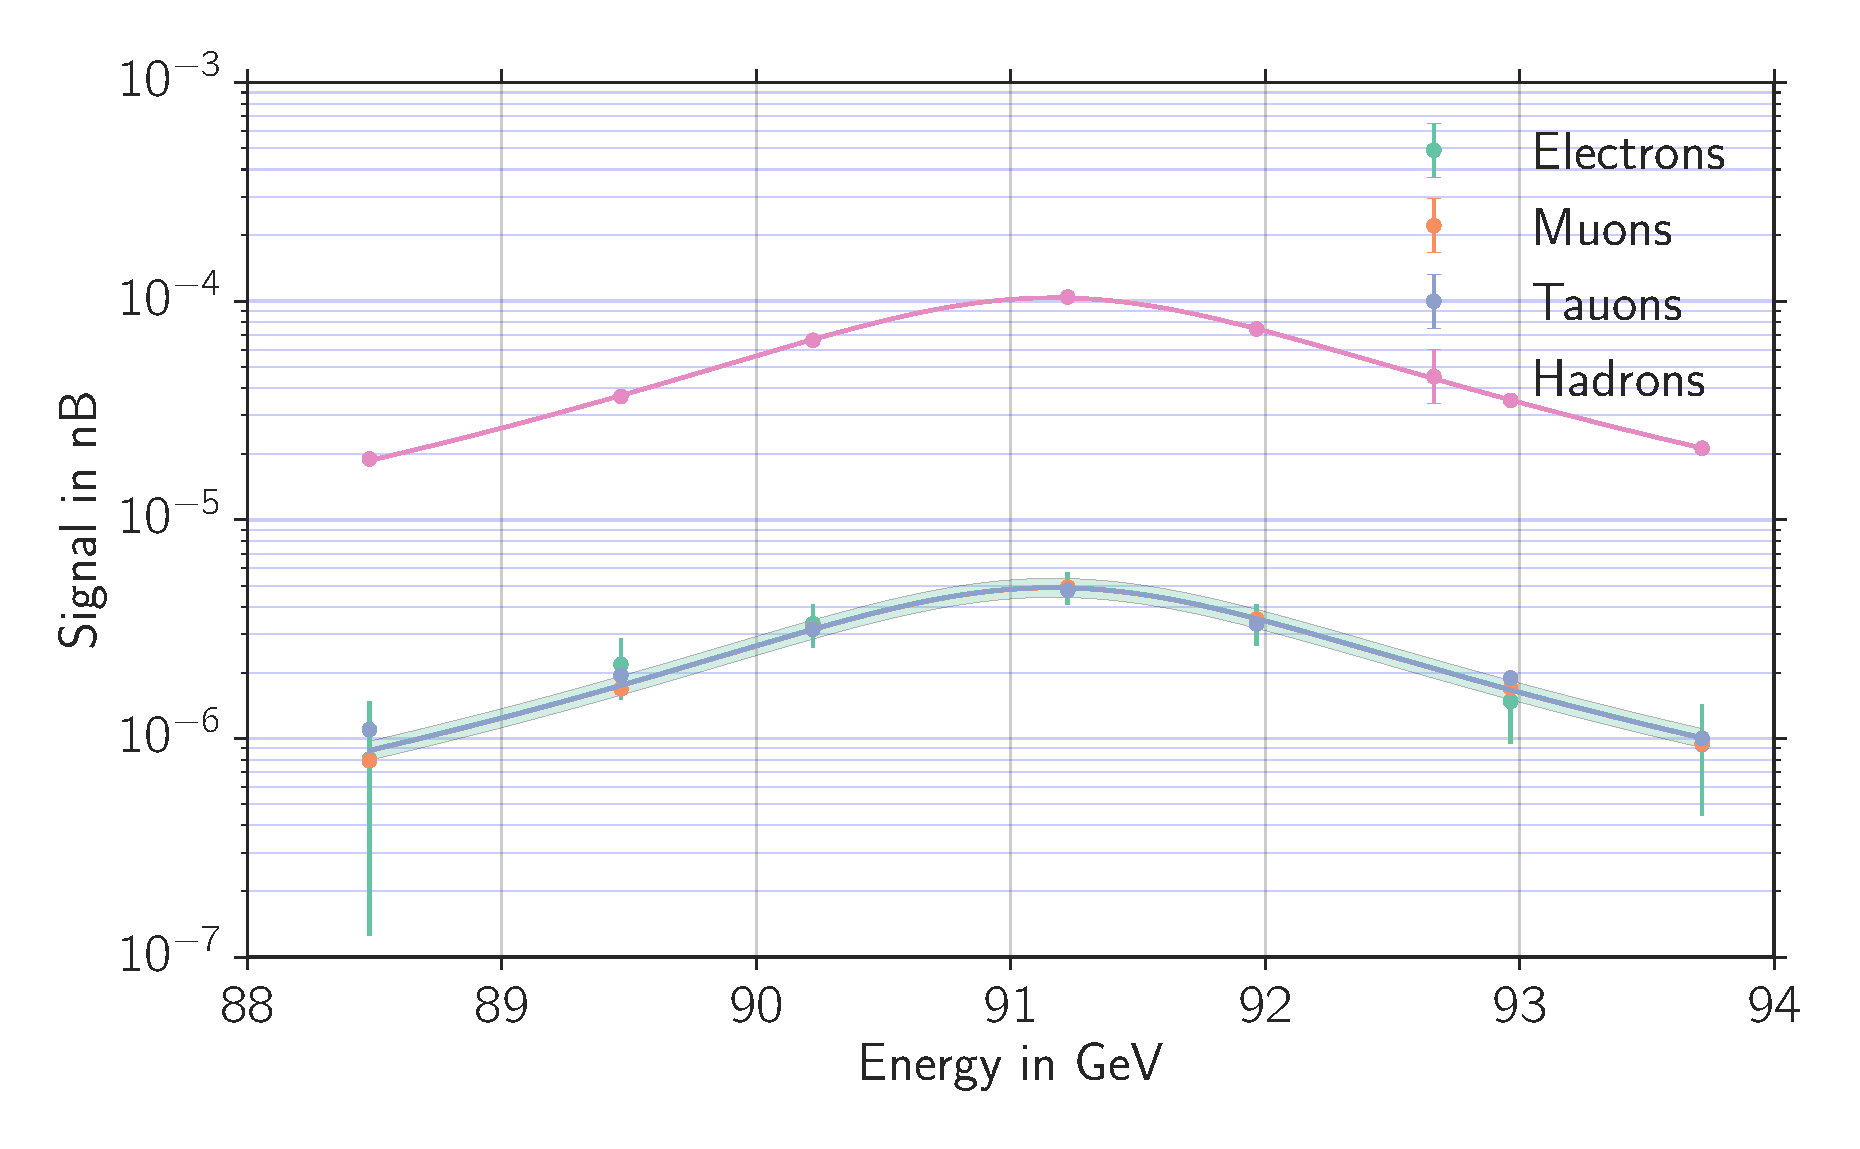
\includegraphics[width=1.0\linewidth]{figures/crosssections}
    \caption{Cross-sections of all particle species. Note that measurement points for 
        muons and tauons are not visible when overlapping with those for electrons. 
        For a more detail picture, see figure \ref{fig:crosssections2} with leptons only
    and figure \ref{fig:crosssections_h} for hadrons only. 
    All four distributions are fitted at once, since they share parameters. 
    }
    \label{fig:crosssections}
\end{figure}


\begin{figure}[htpb]
    \centering
    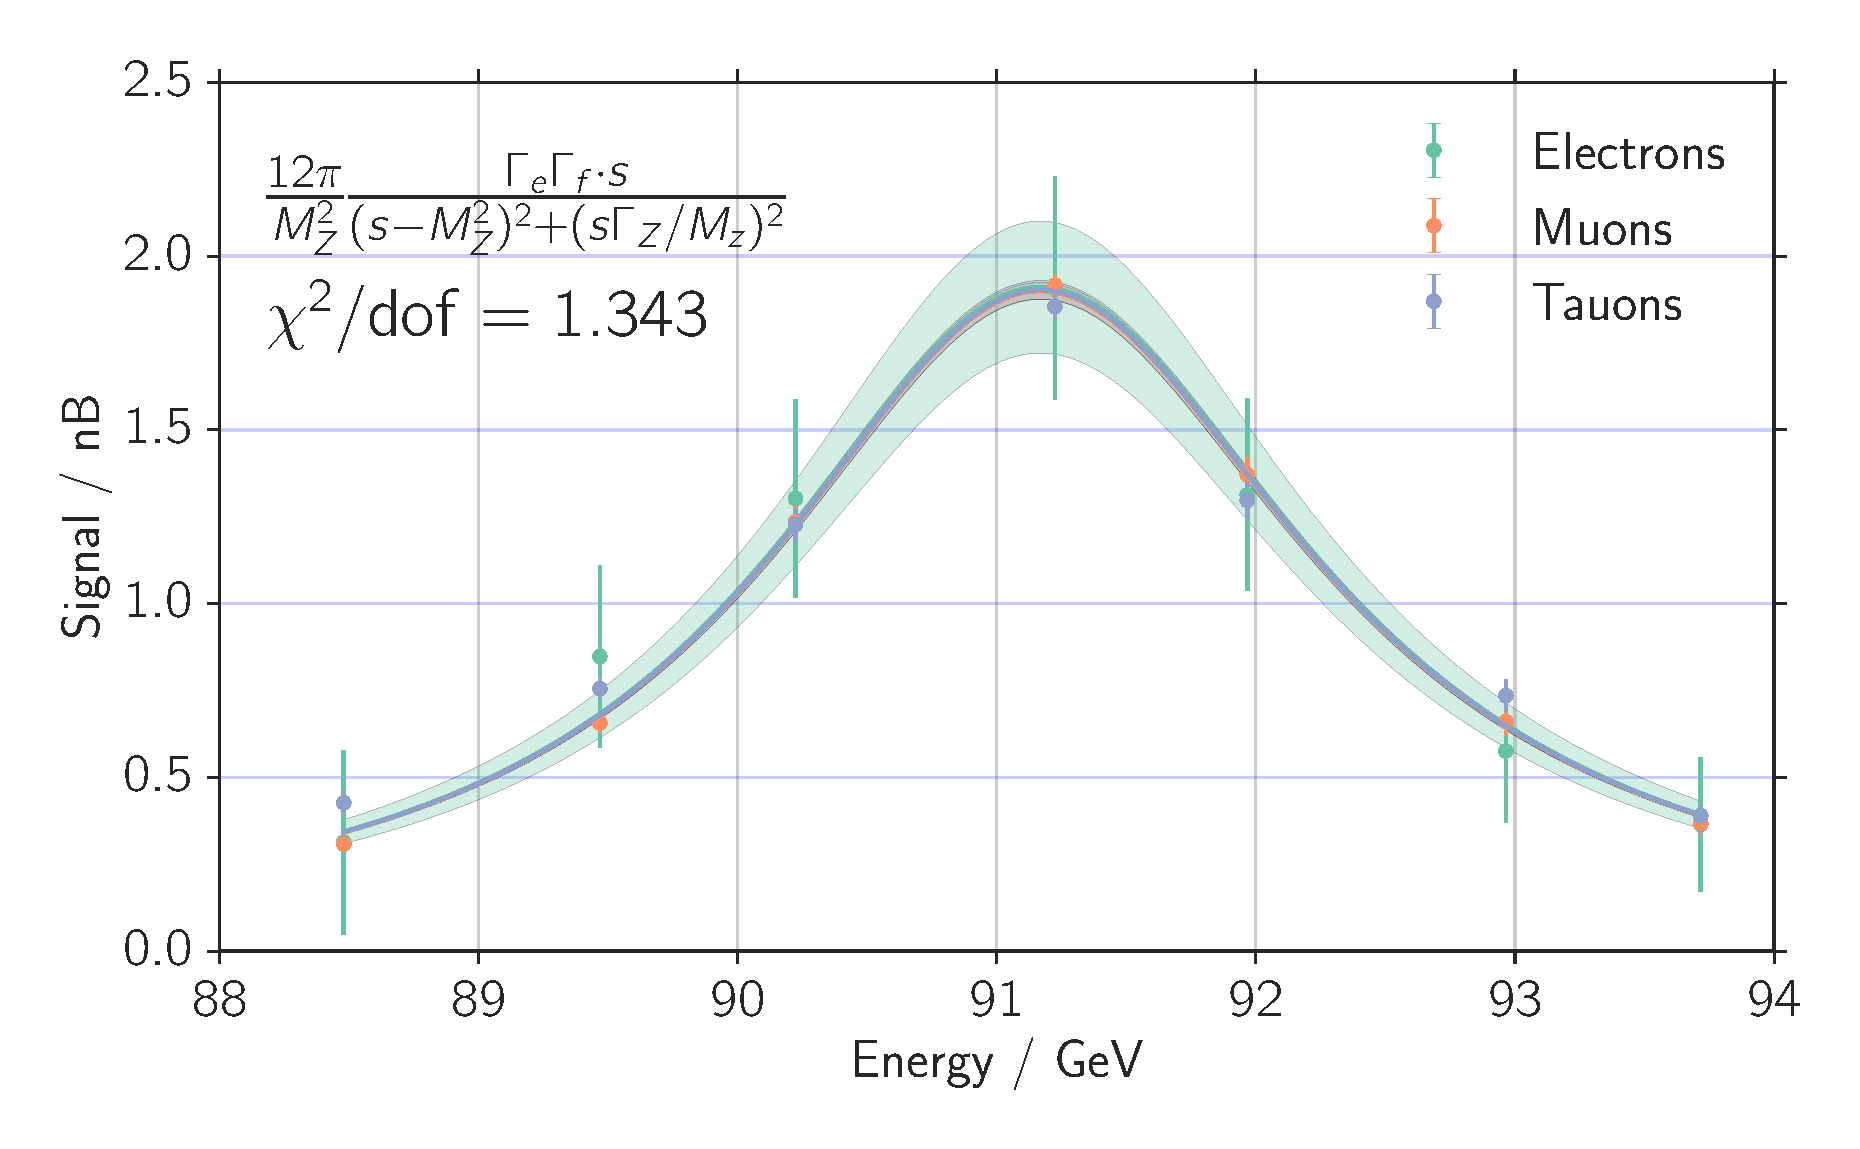
\includegraphics[width=1.0\linewidth]{figures/crosssections2}
    \caption{Cross-sections of leptonic particles on a linear scale. 
        The high error of the electrons is due to the removal of the t-channel which introduces 
        a larger error on the cross sections. 
        For the plot with all particles see figure \ref{fig:crosssections}.
    }
    \label{fig:crosssections2}
    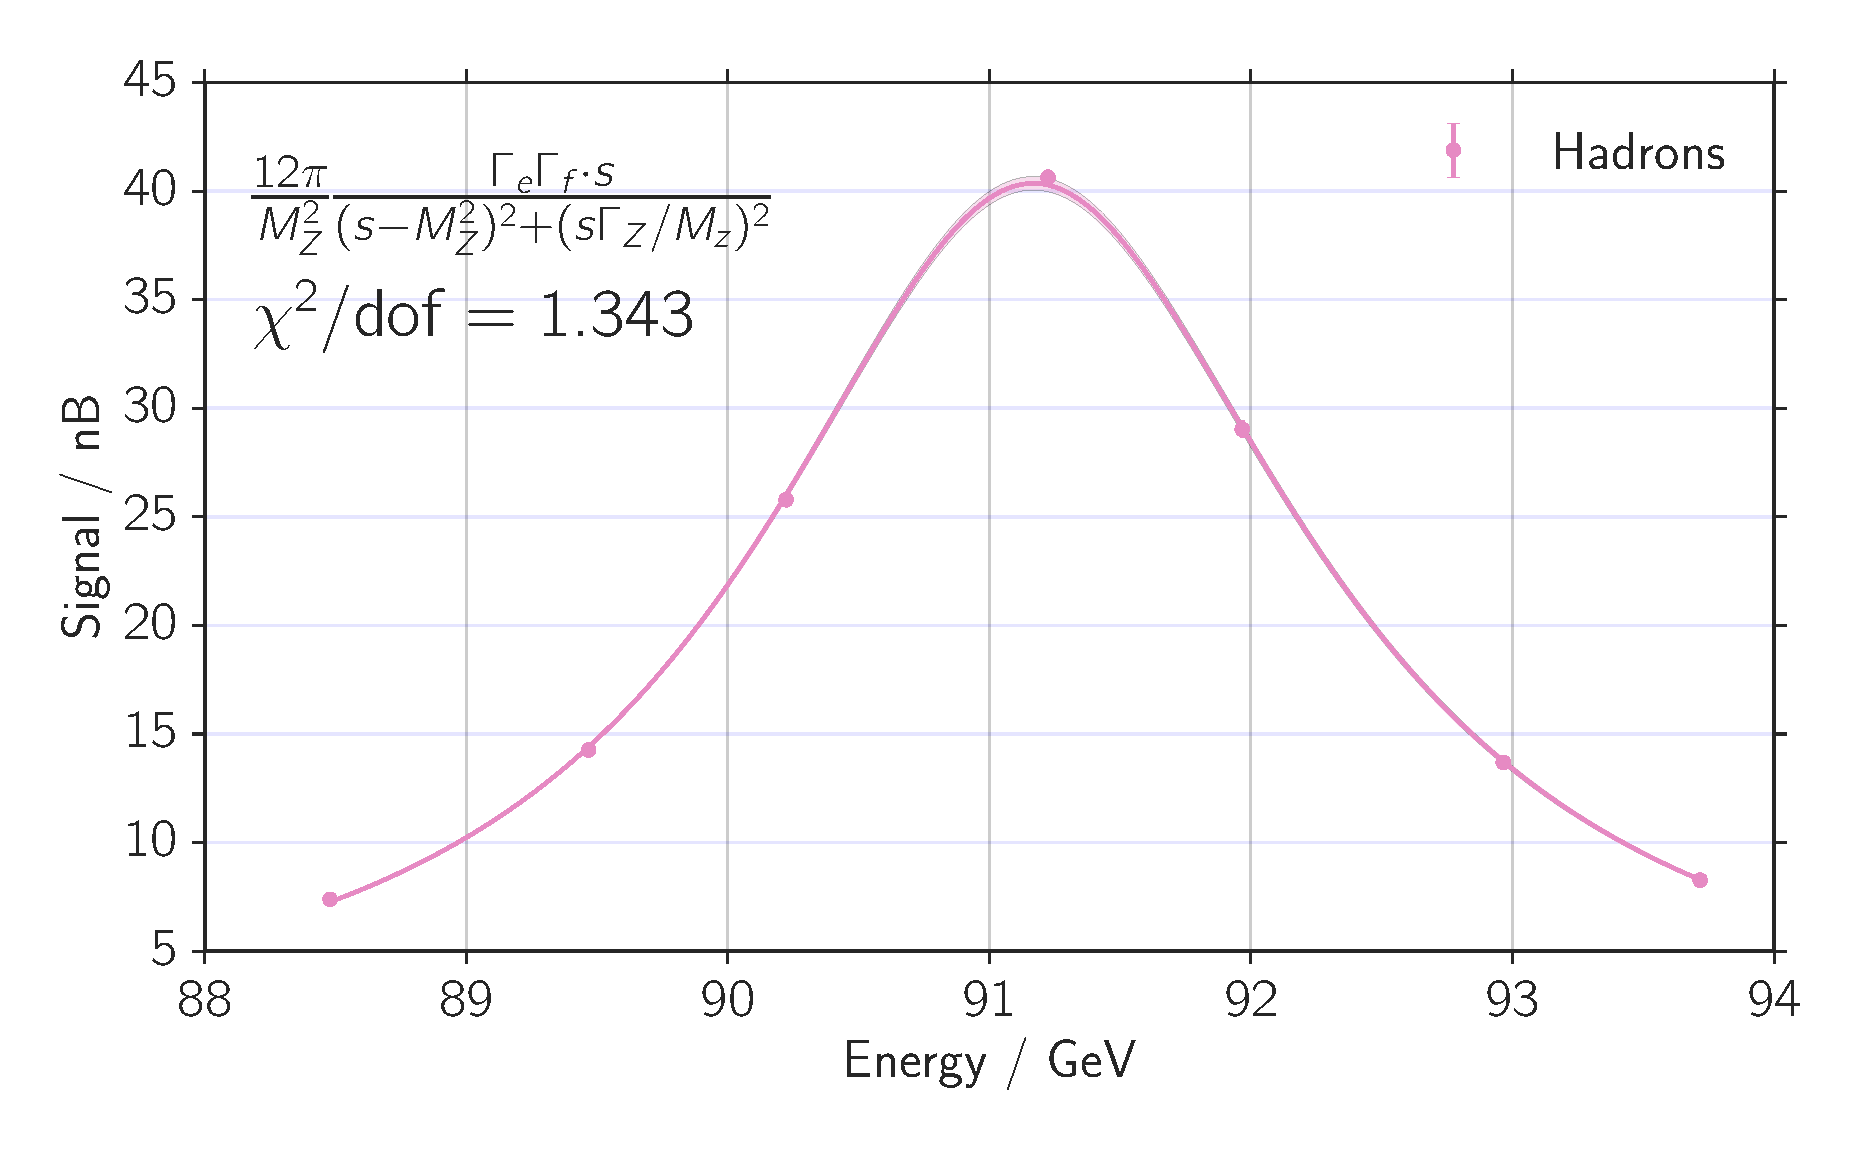
\includegraphics[width=1.0\linewidth]{figures/crosssections_h}
    \caption{Cross-sections of hadrons. Note the different scale in comparison to figure \ref{fig:crosssections2}.
    The value of $\chi^2/\mathrm{dof}$ bigger than one points at either an underestimation
    of uncertainties or their non-Gaussian behavior due to other systematic errors.}
    \label{fig:crosssections_h}
\end{figure}

\begin{table}[htpb]
    \centering
\caption{Results: Partial decay width, width and mass of Z0}
\label{tab:results}
    \begin{tabular}{l l l}
 \rowcolor{LightCyan} & Our result & Literature value \\
 \cellcolor{LightCyan}$\Gamma_e$ / GeV &   $ 0.084\pm0.004   $ & $0.08391 \pm 0.00012 $\\
 \cellcolor{LightCyan}$\Gamma_\mu$ / GeV&   $ 0.084\pm0.004 $ & $0.08399 \pm 0.00018 $\\
 \cellcolor{LightCyan}$\Gamma_\tau$ / GeV&   $ 0.084\pm0.004   $ & $0.08408 \pm 0.00022 $\\
 \cellcolor{LightCyan}$\Gamma_h$ / GeV&   $ 1.78\pm0.90     $ & $1.7444\pm0.002      $\\
 \cellcolor{LightCyan}$\Gamma_Z$ / GeV&   $ 2.558\pm0.020   $ & $2.4952\pm0.0023     $\\
 \cellcolor{LightCyan}$M_Z    $ / GeV /$c^2$&   $ 91.186\pm0.008  $ & $91.187\pm0.0021     $\\
    \end{tabular}
\end{table}

\begin{table}[htpb]
    \centering
    \caption{Correlation matrix for decay widths and Z0 mass 
        Note the high correlation between the lepton widths and between $M_Z$ and $\Gamma_Z$, respectively.}
    \label{tab:covmat}
\begin{tabular}{l| r| r| r |r | r|r}
\rowcolor{LightCyan} & $\Gamma_e$ & $\Gamma_\mu$ & $\Gamma_\tau$ & $\Gamma_h$ &$\Gamma_Z$ & $M_Z$ \\ 
\cellcolor{LightCyan} $\Gamma_e$ & $1.00$ & $-1.00$ & $-1.00$ & $-1.00$ & $-0.13$ & $-0.16$ \\ 
\cellcolor{LightCyan} $\Gamma_\mu$ & $-1.00$ & $1.00$ & $1.00$ & $1.00$ & $0.19$ & $0.18$ \\ 
\cellcolor{LightCyan} $\Gamma_\tau$ & $-1.00$ & $1.00$ & $1.00$ & $1.00$ & $0.19$ & $0.18$ \\ 
\cellcolor{LightCyan} $\Gamma_h$ & $-1.00$ & $1.00$ & $1.00$ & $1.00$ & $0.18$ & $0.18$ \\ 
\cellcolor{LightCyan} $\Gamma_Z$ & $-0.13$ & $0.19$ & $0.19$ & $0.18$ & $1.00$ & $0.48$ \\ 
\cellcolor{LightCyan} $M_Z$ & $-0.16$ & $0.18$ & $0.18$ & $0.18$ & $0.48$ & $1.00$ \\ 
\end{tabular}



\end{table}
\paragraph{\textbf{Lepton universality:}} 
\label{par:lepton_universality} In the theory section (\ref{sub:lepton_universality}) we calculated the decay widths of the various
particle species and found that leptons exhibit a nearly identical
decay width. At this point we use the experimental data to verify this behavior: 
\label{ssub:leptonun}
\begin{align}
    V_\mu = \frac{\Gamma_\mu}{\Gamma_e} = 0.99 \pm 0.1 \\ 
    V_\tau = \frac{\Gamma_\tau}{\Gamma_e} = 1.00 \pm 0.1 
\end{align}
Clearly lepton universality is confirmed within the estimated uncertainties.

\paragraph{\textbf{Number of neutrino generations:}}
\label{par:number_of_neutrino_generations}
As derived in section \ref{sub:number_of_neutrino_generations}, the theory predicts three different neutrino generations.
Let us now look at our experimental data:
\begin{align}
    \label{eq:gen}
    \Gamma_\nu = \Gamma_Z - \Gamma_e - \Gamma_\mu - \Gamma_\tau - \Gamma_h \\ 
    \Gamma_{\nu, \mathrm{theo}} = 0.165 \pm 0.001 \mathrm{GeV} \\ 
    \Rightarrow \frac{\Gamma_\nu}{\Gamma_{nu, \mathrm{theo}}}  = 3.2 \pm 0.6
\end{align}
Thus, the neutrino generation number is confirmed within the standard deviation, 
although we arrive at a relatively high error. This is due to the
correlation of $\Gamma_Z$ and the widths of the fermions and seems reasonable. As we found before, the value for
$\Gamma_Z$ is slightly too high. Plugging in the literature value for $\Gamma_Z$, we would arrive at
\begin{align}
   \frac{\Gamma_\nu}{\Gamma_{nu, \mathrm{theo}}}  = 2.8 \pm 0.6
\end{align}
which confirms our suspicion. However, this does not alter the result of having three generations.

\paragraph{\textbf{Muon forward-backward asymmetry:}}
\label{par:assymetry}
As elaborated in section~\ref{sub:forward_backward_asymmetry},
we can fit the experimental data of the muonic distribution over $\cos\theta$ at the peak of resonance to the following function
(see figure~\ref{fig:asymmetry} for the fitting):
\begin{equation}
    P(\cos\theta) \propto F_1 ( 1+ \cos^2\theta) + 2 F_2 \cos\theta \, .
\end{equation}
with which we can calculate the forward-backward asymmetry%
\footnote{In our calculations we lost the minus sign without being
    able to recover it. Since a negative
asymmetry is physically not conceivable, we added the plus sign in order to fix further calculations.}
to be
\begin{equation}
    A_{FB} = \frac{3 F_2}{4 F_1} = +0.01790 \pm 0.21817.
\end{equation}
The Weinberg angle $\theta_W$ follows with
\begin{equation}
    \sin^2 \theta_W = \frac{1}{4} \left( 1 - \sqrt{ \frac{A_{FB}}{3}} \right)  = 0.23069 \pm 0.11769
\end{equation}
which is a good agreement with the literature value \cite{pdg} of $\sin^2 \theta_W = 0.23126 \pm 0.00005$ within
one standard deviation.


\begin{figure}[htpb]
    \centering
    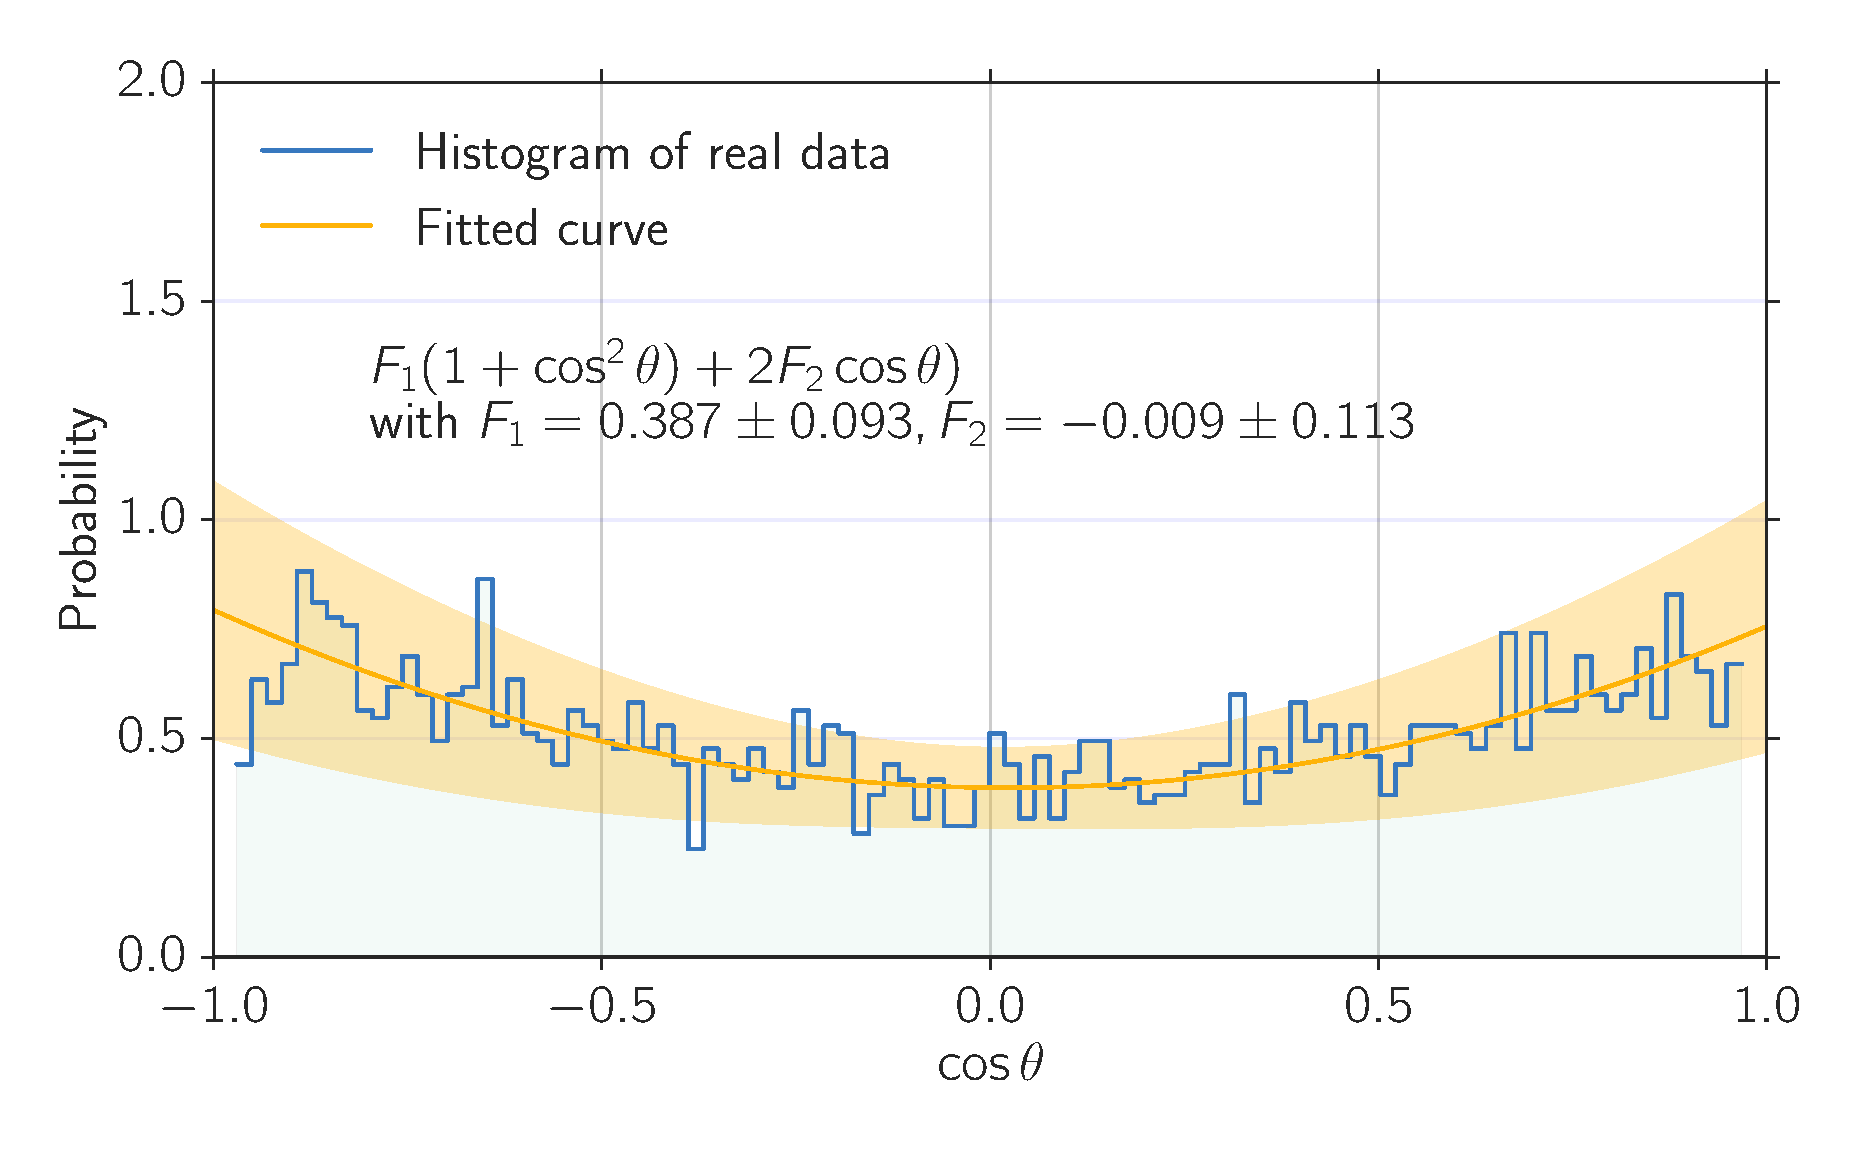
\includegraphics[width=1.0\linewidth]{figures/assymetry}
    \caption{Muon forward-backward asymmetry at peak. As before, 
        the area is the error of the fit, which is in this case much larger than in
    the other fits. The reason for this is the rather huge fluctuation of the data, which is not reflected in the error 
    $\sqrt{N}$, being a rather bad approximation here; this is why the $\chi^2 / \mathrm{dof}$ is much lower than one.
    Further calculations, however, are based on the large errors induced by the fluctuations.
}
    \label{fig:asymmetry}
\end{figure}

